% !TEX root =  ../pers_schedules.tex 

\section{Simulation study}
\label{sec: simulation_study}
The application of personalized schedules for patients from PRIAS demonstrated that the schedules adapt according to the historical data of each patient. However we could not perform a full scale comparison between personalized and PRIAS schedules, because the true time of GR was not known for any of the PRIAS patients. To this end, we have performed a simulation study comparing personalized schedules based on expected time of GR, median time of GR and dynamic risk of GR with a mixed approach between median time of GR and dynamic risk of GR, PRIAS schedule and annual schedule. We employ these schedules for simulated patients enrolled in a hypothetical AS program, with the same entrance criteria as PRIAS.

\subsection{Simulation setup}
\label{subsec : simulation_setup}
\subsubsection{Patient population}
First we assume a population of patients enrolled in AS, whose PSA and hazard of GR follows a joint model of the form postulated in Section \ref{subsec : jm_fit_prias}, with parameters equal to the posterior mean of parameters (CHECK WEB SUPPLEMENTARY SECTION...) estimated from the joint model fitted to PRIAS dataset. We assume that the patients in population belong to 3 equal sized subgroups $G_1, G_2, G_3$ with different failure times. The failure times are controlled by different Weibull distributed baseline hazards for each. The shape and scale parameters $(k, \lambda$) for the 3 subgroups are: $(1.5, 4)$, $(3, 5)$ and $(4.5, 6)$ for $G_1, G_2$ and $G_3$ respectively. The effect of these parameters is that the variance in GR times is highest for $G_1$ and lowest for $G_3$, while the mean GR time is lowest in $G_1$ and highest in $G_3$.

From the population we randomly sample a total of 408 datasets with 1000 patients each. Each dataset is split into a training (750 patients) and a test (250 patients) part. The $k$-th simulated training dataset $\mathcal{D}^k$ is given by $\mathcal{D}^k = \{l_{ki}, r_{ki}, \boldsymbol{y}_{ki}; i = 1, \ldots, 750\}$, where $\boldsymbol{y}_{ki}$ denote the PSA measurements for the $i$-th patient in $\mathcal{D}^k$. The frequency of PSA measurements is same as that in PRIAS. Other than simulating a true GR time $T^*_{ki}$, we also generate a random and non-informative censoring time $C_{ki}$. When $T_{ki} < C^*_{ki}$, then $l_{ki} = r_{ki} = T^*_{ki}$, otherwise $l_{ki} = C_{ki}$ and $r_{ki} = \infty$. For the test patients, censoring time is not generated.

Next we fit a joint model of the specification given in \ref{eq : long_model_prias} and \ref{eq : hazard_prias} to each of the $\mathcal{D}^k, k=1,
\ldots, 408$, and obtain posterior distribution of parameters $p(\boldsymbol{\theta} \mid \mathcal{D}^k)$. Using the latter, we obtain the PPD $g(T^*_{kj})$ for the $j$-th test patient and conduct hypothetical biopsies iteratively in accordance with the algorithm in Figure \ref{fig : sched_algorithm}. 

\subsection{Estimation}
For estimation of the optimal $\kappa = \argmax_{\kappa} F_1(t, \Delta t, s)$, we use a grid search approach. That is, $F_1$ is computed using the training dataset over a fine grid of $\kappa$ values in the interval $[0,1]$  and then the most optimal value is chosen.

The next step is to estimate the measures of efficacy of schedules. To this end, we estimate $E[N^{bS}]$, $\mbox{var}[N^{bS}]$, $E[O^S]$ and $\mbox{var}[O^S]$ using pooled estimates of each from the 408 test datasets, as follows:
\begin{align*}
\widehat{E[O^S]} &= \frac{\sum_{k=1}^{254} n_k \widehat{E[O^S_k]}}{\sum_{k=1}^{254} n_k}, \\
\widehat{\mbox{var}[O^S]} &= \frac{\sum_{k=1}^{254} (n_k - 1) \widehat{\mbox{var}[O^S_k]}}{\sum_{k=1}^{254} (n_k-1)}, 
\end{align*}
where $n_k$ are the number of test patients in the $k$-th simulation, $\widehat{E[O^S_k]} = {\sum_{j=1}^{n_k}O^S_{kj}}/{n_k}$ is the estimated mean and $\widehat{\mbox{var}[O^S_k]} = {\sum_{j=1}^{n_k}\big\{O^S_{kj} - \widehat{E[O^S_k]}\big\}^2}/{n_k-1}$ is estimated variance of the offset for the $k$-th simulation. The estimates for number of biopsies $N^{bS}$ are obtained similarly.

\subsection{Results}
From the simulations we calculated the pooled estimates of the mean and variance of number of biopsies/offset for the entire sample. The estimates are plotted in Figure \ref{fig : meanNbVsOffset} and also summarized in Table \ref{table : sim_study_pooled_estimates}. From the figure it is evident that those schedules which conduct less biopsies on average, have a higher average offset, and vice versa. For example, the annual schedule conducts 5.2 biopsies on average, which is the highest among all schedules, however it has the least average offset of 6 months as well. On the other hand the schedule based on expected time of GR conducts only 1.9 biopsies on average, the least among all schedules but it also has the highest average offset of 15 months. The schedule based on median time of GR performs almost the same as that based on expected time of GR. As mentioned earlier the variance in number of biopsies and offset are important as well. In this regard annual schedule has the largest $\mbox{var}[N^{bS}]$ since it attempts to contain the offset within an year, and consequently it has the least $\mbox{var}[O^S]$. Schedules based on expected and median time of GR perform the opposite in terms of variance.

\begin{figure}
	\centerline{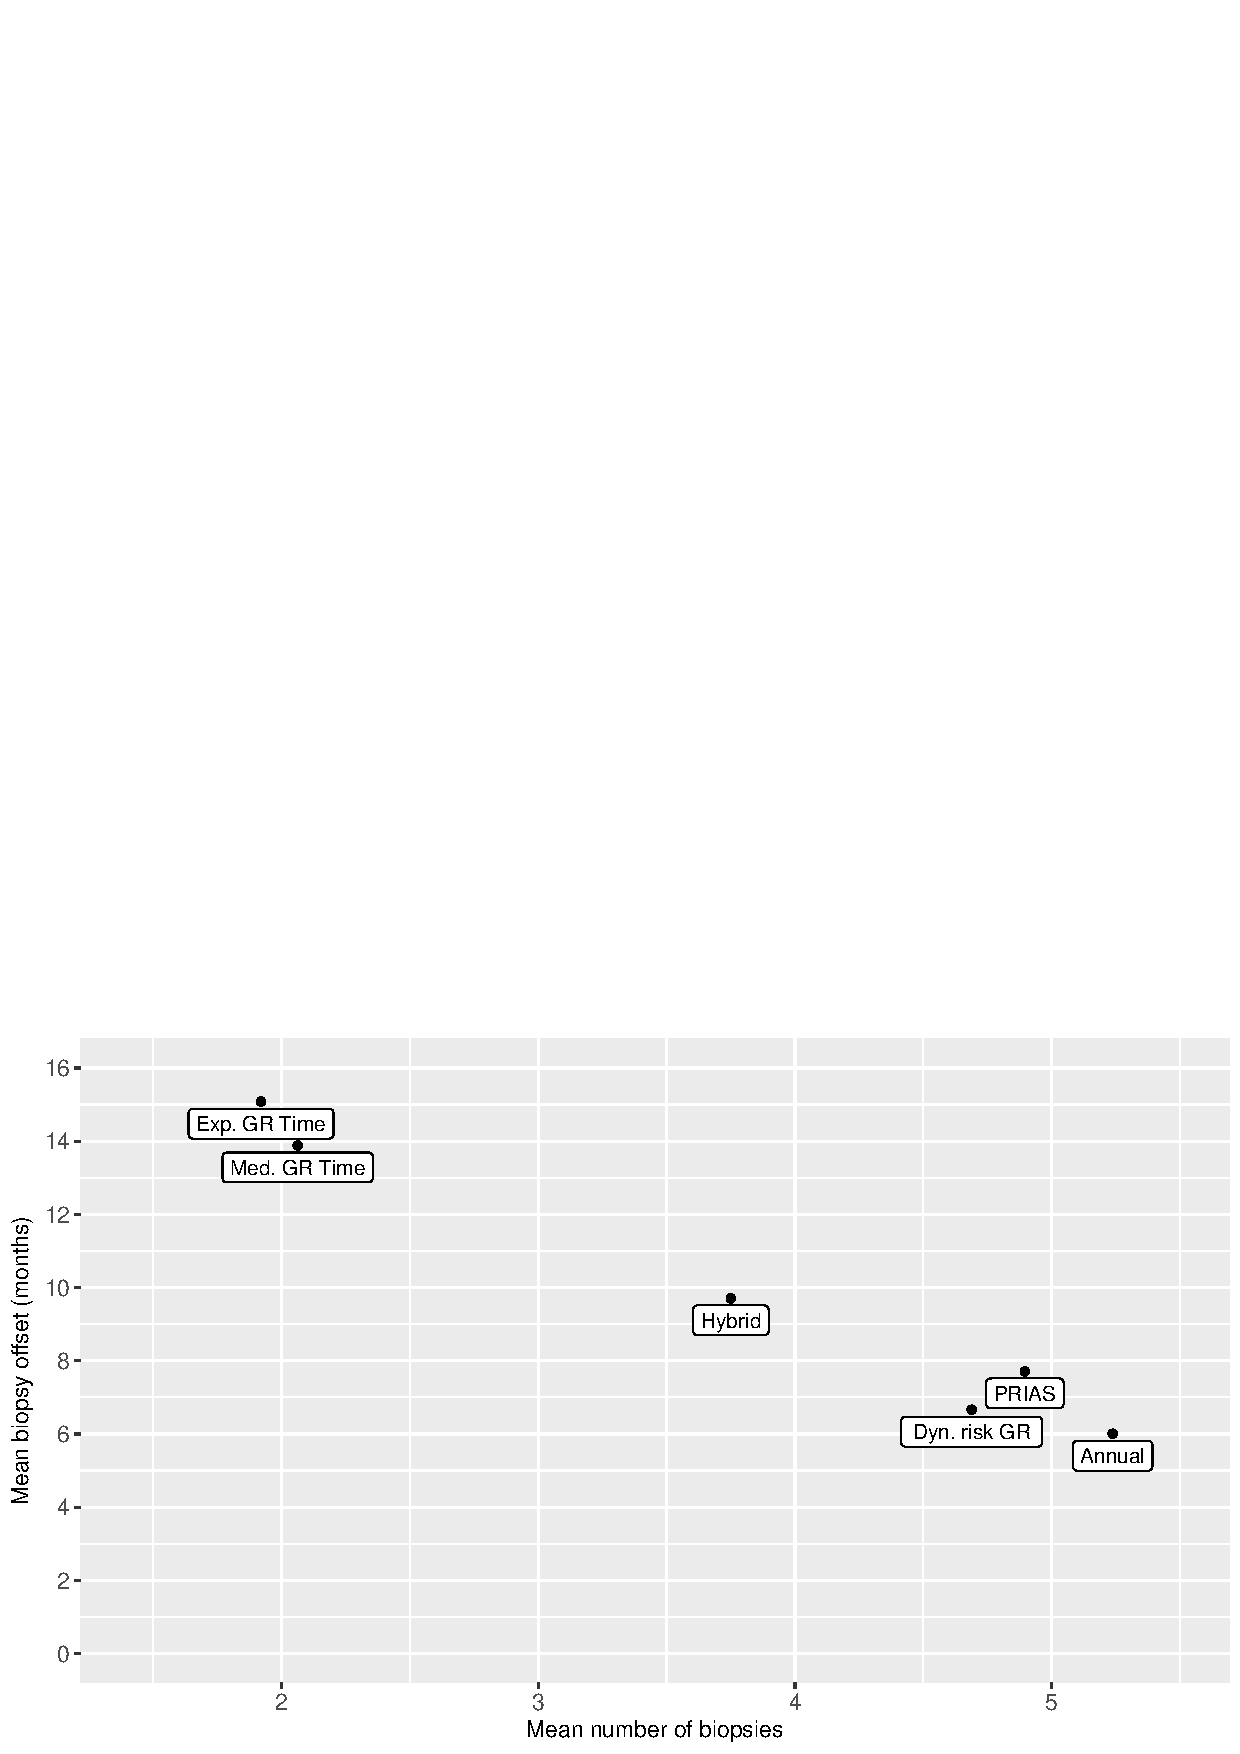
\includegraphics[width=\columnwidth]{images/sim_study/meanNbVsOffset_all.png}}
	\caption{Estimated mean number of biopsies and mean offset (months) for the 7 scheduling methods using all patients. Method names are abbreviated for ease of graphing.}
	\label{fig : meanNbVsOffset}
\end{figure}

\begin{table}
\caption{Pooled estimates of mean and variance of number of biopsies and offset for all patients.}
\label{table : sim_study_pooled_estimates}
\begin{tabular}{lrrrr}
\Hline
Schedule          & $E[N^{bS}]$ & $E[O^{S}]$ & $\mbox{var}[N^{bS}]$ & $\mbox{var}[O^S]$ \\  \hline
Annual & 5.23           & 6.00               & 6.42          & 11.87             \\
PRIAS & 4.85           & 8.46               & 5.52          & 74.22             \\
Expected time of GR & 1.92           & 15.06              & 1.42          & 146.31          \\
Median time of GR  & 2.06           & 13.89              & 2.00          & 139.73            \\
$\text{F}_1$-Score  & 4.68           & 6.65               & 4.80          & 18.83             \\
Mixed approach & 3.76          & 9.74               & 2.88          & 58.35             \\
\hline
\end{tabular}
\end{table}

We observe that the PRIAS schedule performs more or less the same as annual schedule. Despite this the latter may be preferred over PRIAS since it conducts only 0.38 biopsies more on average, however unlike PRIAS it has very low variance of offset, thus guaranteeing early detection for everyone. If we compare the PRIAS schedule with dynamic risk of GR based schedules, we can see that the schedule where $\kappa$ is chosen after maximizing $\text{F}_1$-Score, performs better than in PRIAS schedule in all aspects. The schedule where $\kappa$ is chosen after maximizing Youden's $J$ has a very large $\mbox{var}[O^S]$ and hence is not preferable over PRIAS. The mixed approach combines the benefits of methods with low $E[N^{bS}]$ and $\mbox{var}[N^{bS}]$, and those methods with low $E[O^{S}]$ and $\mbox{var}[O^S]$. It conducts 1.5 less biopsies than annual schedule on average and at 9.7 months the mean offset is less than an year.

\begin{table}
\caption{Pooled estimates of mean and variance of number of biopsies and offset for subgroup $G_1$.}
\label{table : sim_study_pooled_estimates_G1}
\begin{tabular}{lrrrrr}
\Hline
Schedule           & Total Patients & $E[N^{bS}]$ & $E[O^{S}]$ & $\mbox{var}[N^{bS}]$ & $\mbox{var}[O^S]$ \\  \hline
Annual              & 21004                  & 4.306           & 6.024               & 9.788          & 11.747             \\
PRIAS              & 21004                  & 4.032           & 7.951               & 8.221          & 63.528             \\
Expected time of GR & 21001                  & 1.922           & 15.114              & 1.441          & 149.167            \\
Median time of GR  & 20937                  & 2.068           & 13.87               & 1.999          & 138.396            \\
$\text{F}_1$-Score           & 21061                  & 4.689           & 6.648               & 4.863          & 18.745             \\
Mixed approach     & 21004                  & 3.252           & 10.361              & 4.611          & 73.781             \\
\hline
\end{tabular}
\end{table}

\begin{table}
\caption{Pooled estimates of mean and variance of number of biopsies and offset for subgroup $G_2$.}
\label{table : sim_study_pooled_estimates_G2}
\begin{tabular}{lrrrrr}
\Hline
Schedule           & Total Patients & $E[N^{bS}]$ & $E[O^{S}]$ & $\mbox{var}[N^{bS}]$ & $\mbox{var}[O^S]$ \\  \hline
Annual              & 21160                  & 5.181           & 5.95                & 4.567          & 12.03              \\
PRIAS              & 21160                  & 4.817           & 8.569               & 3.98           & 75.716             \\
Expected time of GR & 21151                  & 1.927           & 15.078              & 1.447          & 144.333            \\
Median time of GR  & 21189                  & 2.062           & 13.947              & 1.994          & 140.633            \\
$\text{F}_1$-Score           & 21133                  & 4.666           & 6.663               & 4.726          & 18.956             \\
Mixed approach     & 21160                  & 3.702           & 10.359              & 1.869          & 60.415             \\
\hline
\end{tabular}
\end{table}

\begin{table}
\caption{Pooled estimates of mean and variance of number of biopsies and offset for subgroup $G_3$.}
\label{table : sim_study_pooled_estimates_G3}
\begin{tabular}{lrrrrr}
\Hline
Schedule           & Total Patients & $E[N^{bS}]$ & $E[O^{S}]$ & $\mbox{var}[N^{bS}]$ & $\mbox{var}[O^S]$ \\  \hline
Annual              & 21222                  & 6.214           & 6.03                & 3.118          & 11.851             \\
PRIAS              & 21222                  & 5.717           & 8.866               & 2.977          & 82.915             \\
Expected time of GR  & 21234                  & 1.921           & 15.006              & 1.375          & 145.426            \\
Median time of GR   & 21260                  & 2.07            & 13.879              & 2.016          & 140.14             \\
Youden's $J$              & 21202                  & 4.541           & 8.02                & 4.061          & 112.559             \\
Mixed approach     & 21222                  & 4.33            & 8.521               & 1.581          & 38.586             \\
\hline
\end{tabular}
\end{table}

We next check the performance of these methods for each of the 3 subgroups $G_1, G_2$ and $G_3$. Estimates of $E[N^{bS}]$, $\mbox{var}[N^{bS}]$, $E[O^S]$ and $\mbox{var}[O^S]$ for the 3 subgroups are presented in Table \ref{table : sim_study_pooled_estimates_G1}, Table \ref{table : sim_study_pooled_estimates_G2} and Table \ref{table : sim_study_pooled_estimates_G3}. We observe that all of the schedules which are based on personalized methods, i.e. expected time of GR, median time of GR and dynamic risk of GR based schedules perform the same across the subgroups, with trivial differences in estimates. On the other hand, the annual schedule conducts 6 biopsies on average for patients in $G_3$ as compared to 4 for patients in $G_1$. It also has $\mbox{var}[N^{bS}]$ 3 times more for patients in $G_1$ compared to $G_3$. This can be attributed to the former having higher variance in GR times. However for annual schedule the $E[O^S]$ and $\mbox{var}[O^S]$ remain almost the same in all groups and it always detects GR within an year of the occurrence. The PRIAS schedule differs for the 3 subgroups as well. For number of biopsies the dynamics are similar to that of annual schedule. However for offset, the PRIAS schedule has high $E[O^S]$ and $\mbox{var}[O^S]$ for patients from $G_3$, i.e. patients who obtain GR later. As for the mixed approach, we observe that it conducts more biopsies on average for patients from $G_3$, however it also has the least $E[O^S]$, $\mbox{var}[O^S]$ and $\mbox{var}[N^{bS}]$ for the same group.

To assess the methods further, we combined data from all of the 63386 patients, and also plotted the box plots for number of biopsies and offset in Figure \ref{fig : nbBoxPlot} and Figure \ref{fig : offsetBoxPlot} respectively. Based on the combined data, we observe that both expected and median failure time of GR based schedules have 91.7\% and 92.5\% of patients below offset cutoff of 36 months, respectively. They also have 80.5\% and 82.3\% of patients below a cutoff of 24 months. Thus they seem to be quite practical. The mixed approach offers another practically viable solution, since neither it has large $\mbox{var}[N^{bS}]$, nor $\mbox{var}[O^S]$. The estimated $E[N^{bS}]$ is 3.8 and the estimated $E[O^S]$ is 9.7 months. For 99.9\% patients it has an offset below 36 months and for 95\% patients it has an offset below 24 months. Given this offset and the fact that it conducts much less biopsies than PRIAS schedule, annual schedule, and dynamic risk of GR based schedules, it is preferable over them.